\documentclass[a4paper,12pt,english]{report}
\usepackage{wrapfig}
\usepackage{graphicx}
\usepackage{listings}
\usepackage{hyperref}
\usepackage{etoolbox}
\usepackage{titlesec}
\lstset{ %
basicstyle=\footnotesize,       
frame=single,          
}

\titleformat{\chapter}[display]
  {\normalfont\bfseries}{}{0pt}{\Huge}
\titlespacing*{\chapter}{0pt}{-50pt}{40pt}
	
\newcommand*{\titleGM}{\begingroup 
\hbox{
\hspace*{0.2\textwidth} 
\rule{1pt}{\textheight} 
\hspace*{0.05\textwidth} 
\parbox[b]{0.75\textwidth}{ 

{\noindent\Huge\bfseries User Manual}\\[2\baselineskip]
{\large \textit{Visan - Visual data analysis package}}\\[4\baselineskip] 
{\Large \textsc{Ramzan Umarov and Victor Solovyev}}

\vspace{0.5\textheight} 
{\noindent April, 2017}\\[\baselineskip] 
}}
\endgroup}

\begin{document}
\titleGM 
\thispagestyle{empty}
\newpage
\tableofcontents
\thispagestyle{empty}
\newpage

\pagenumbering{arabic}
\section*{Introduction}
\addcontentsline{toc}{section}{Introduction}
VISAN can create, save and open projects. Save project is used to save the data set, the decision thresholds for classification methods, and also the neural networks if any were created. To save project press save icon or File/Save menu. Then navigate to place where you want to save the project, enter the project name and press save. 

\begin{figure}[htb]
\centering
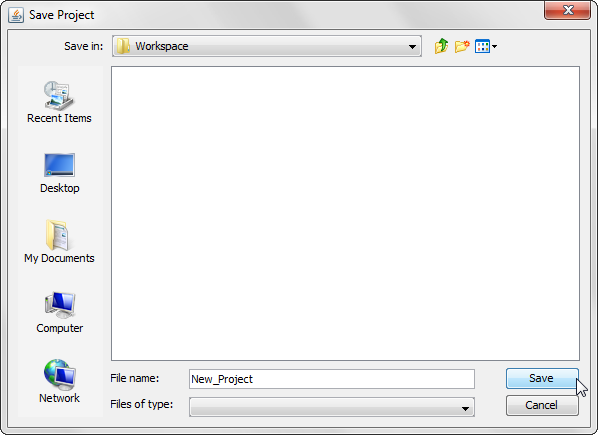
\includegraphics[width=240pt]{save.png}
\caption{Saving Project}
\end{figure}


Folder with the project name will be created. In that folder there will be a file with the project name and extension "vis". Now the saved project can be opened by opening that file. However, it is not necessary. You can work with the program without ever saving the project.

To start working user first needs to load data; this can be done from menu Data/Load Learning Set or by pressing the "load data" icon. 

\begin{figure}[htb]
\centering
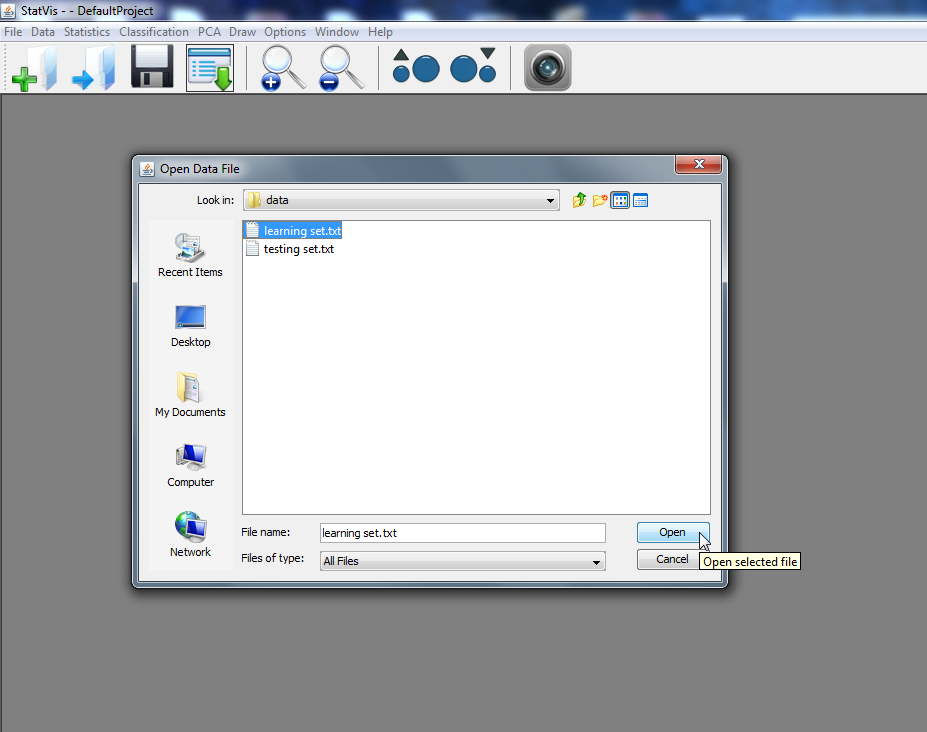
\includegraphics[width=320pt]{s1.png}
\caption{Loading Data}
\end{figure}
\newpage


User will be asked what delimiter to use and where the class label is located. If data is delimited with tab or space leave the field blank. 


\begin{figure}[htb]
\centering
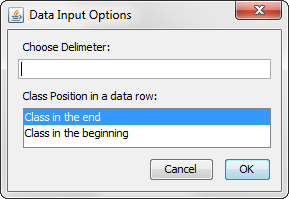
\includegraphics[width=160pt]{s2.png}
\caption{Data Input Options}
\end{figure} 


After reading in the data, you will be prompted for negative class, if it is unknown or not needed just press OK.
\newpage
\section*{Data Structure}
Data can have features names included which is indicated by "/features" in the beginning. Then there should be list of objects with the class of object in the end or beginning. 

Example of data with two classes:

\begin{lstlisting}
/features m1 m2 m3 m4 m5 m6   m7 m8 
0.50    0.40    0.45    0.51    0.36    0.41   18.00    0.10 -1 
0.50    0.69    0.57    0.53    0.64    0.74   18.00    0.54  1   
0.48    0.30    0.25    0.48    0.43    0.47   15.00    0.47 -1
0.48    0.16    0.43    0.49    0.43    0.46   11.00    0.38 -1
0.40    0.32    0.36    0.52    0.42    0.52   11.00    0.45 -1
0.45    0.18    0.56    0.52    0.45    0.51   11.00    0.41 -1
0.47    0.32    0.60    0.52    0.28    0.44   20.00    0.40 -1
0.55    0.57    0.31    0.47    0.25    0.42   25.00    0.34 -1
0.34    0.27    0.49    0.51    0.43    0.60   11.00    0.22 -1
0.38    0.16    0.35    0.51    0.42    0.60    7.00    0.37 -1
0.45    0.24    0.62    0.48    0.36    0.48   15.00    0.49 -1  
\end{lstlisting}

\begin{wrapfigure}{L}{5cm} 
\begin{center}
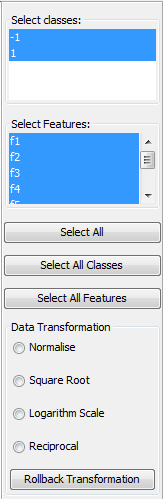
\includegraphics[width = 75pt]{s3.png}
\end{center}
\caption{Data Panel}
\end{wrapfigure}

Before visualizing or analyzing the data, you first need to select classes and features you want to work with. By default, they are all selected (see figure 4). When using classification it is recommended to select all features for best results. However, this is not always the case, since user might want to check importance of each feature, and in some cases feature might not improve the training at all. 

Data can be transformed to improve classification or change its visualization. Select one of the available options: normalize, square root, logarithm scale, and reciprocal. Normalization is crucial for neural networks to work with some data (when features are scaled very differently), but in some cases it may cause classification to work worse. It is recommended to try both.

You can get data statistics which are available from menu Statistics/Descriptive statistics. This will display descriptive statistics for selected features and classes. Important statistics about data are shown such as mean, standard deviation,  and distribution.

\newpage
\section*{Data Visualization}
\addcontentsline{toc}{section}{Data Visualization}

Data can be visualized using following types of graphs: plot, histogram, and trend. Simply select classes, features and type of graph from menu Draw. If you draw plot you can select points and create new class from them using menu Data/Start Selection and then Data/Finish. Left click to select point nearest to where you clicked and right click to select multiple points by drawing closed shape:

\begin{figure}[htb]
\centering
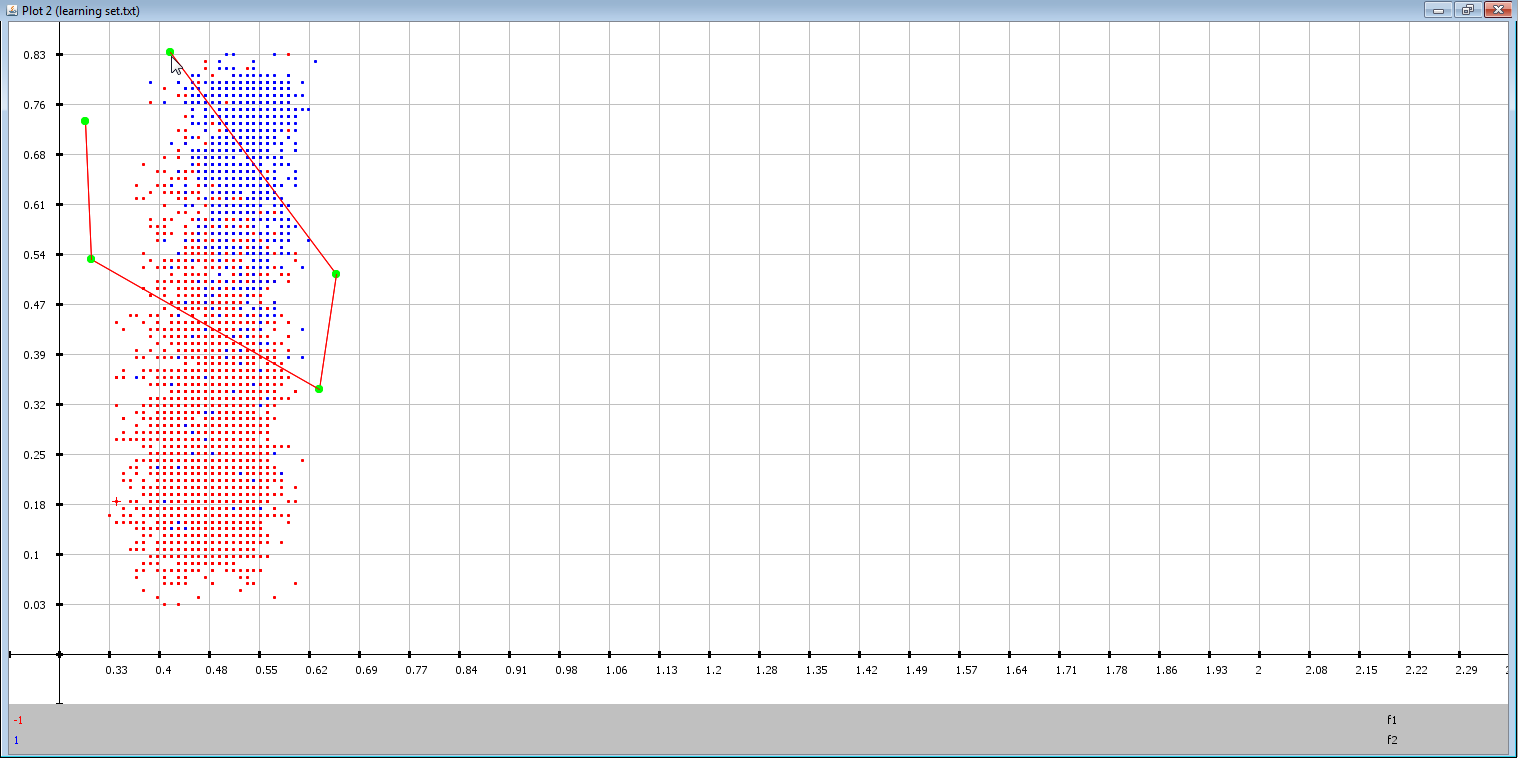
\includegraphics[width=320pt]{s4.png}
\end{figure}

Right click on the first point to finish selection:

\begin{figure}[htb]
\centering
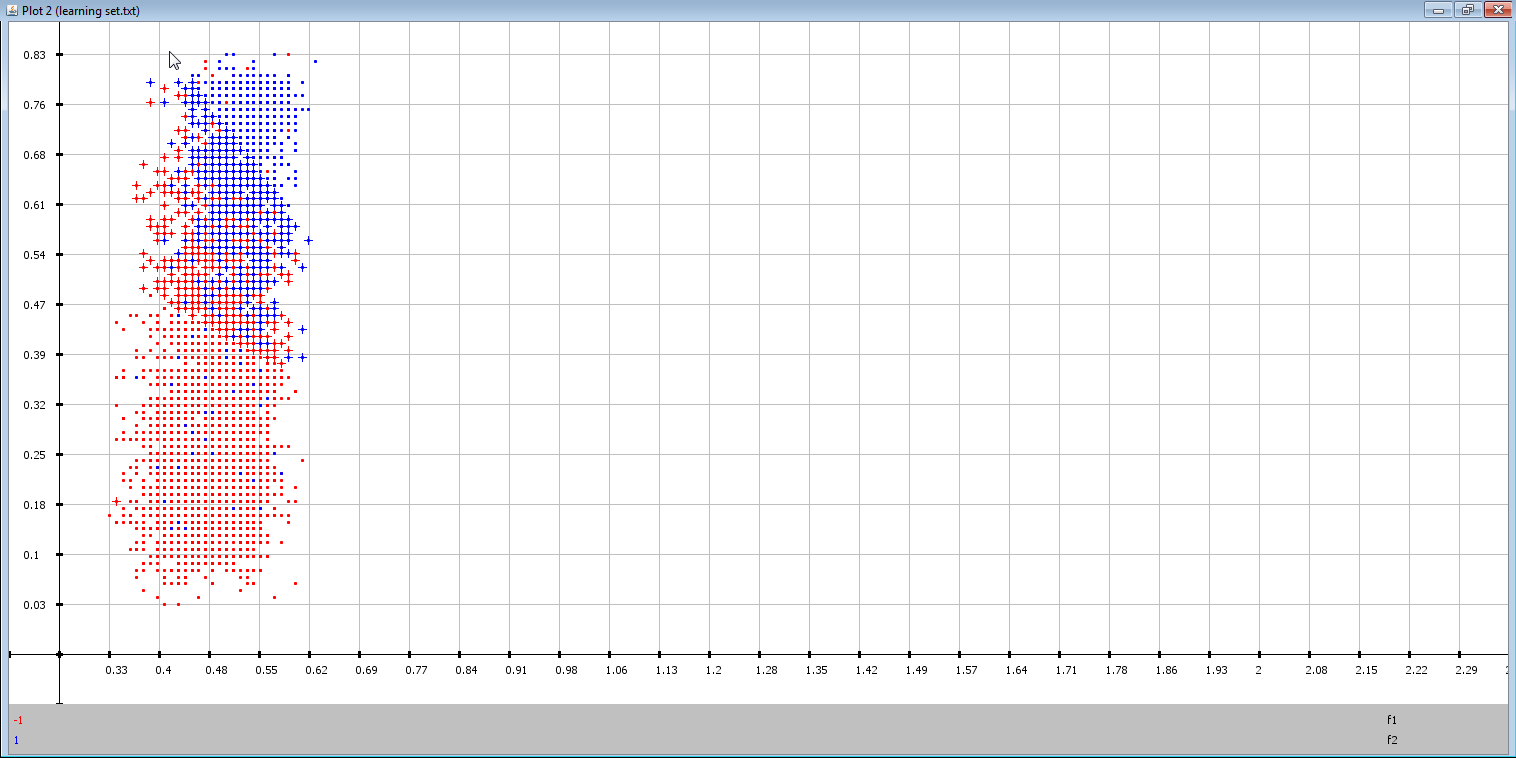
\includegraphics[width=320pt]{s5.png}
\end{figure}
 


\newpage
You can change the number of bins of the histogram and its type in options menu (Options/Histogram Options/Number Of Bins). Use tools panel to increase and decrease point size, zoom in and zoom out, and also to take snapshots of your graphs.



Histogram of feature m1 with number of bins set to 10:
 
\begin{figure}[htb]
\centering
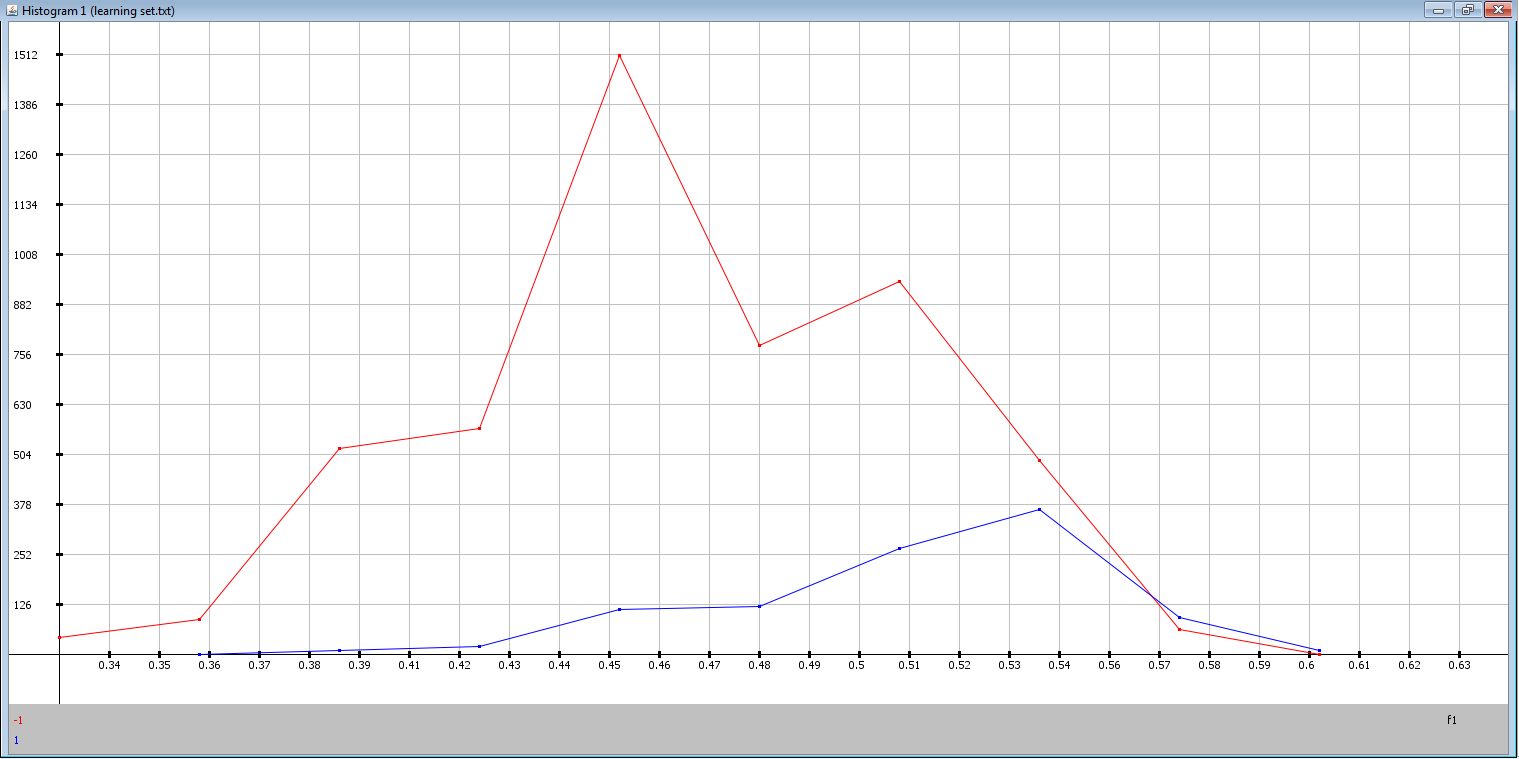
\includegraphics[width=260pt]{s6.png}
\end{figure} 
 
 
 
Histogram of feature m1 with number of bins set to 25:
 
 
 
\begin{figure}[htb]
\centering
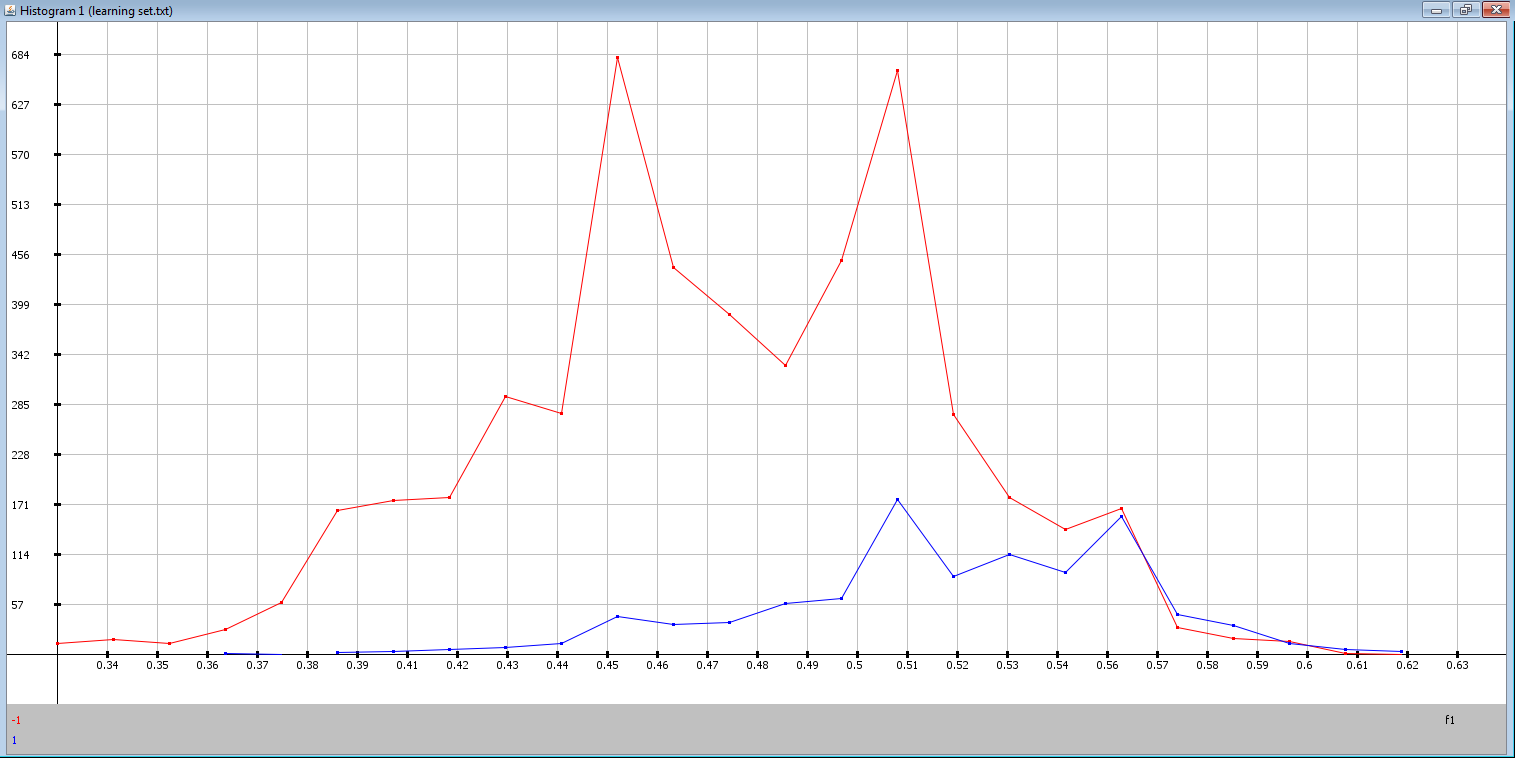
\includegraphics[width=260pt]{s7.png}
\end{figure} 



Another type of histogram for the same data:



\begin{figure}[htb]
\centering
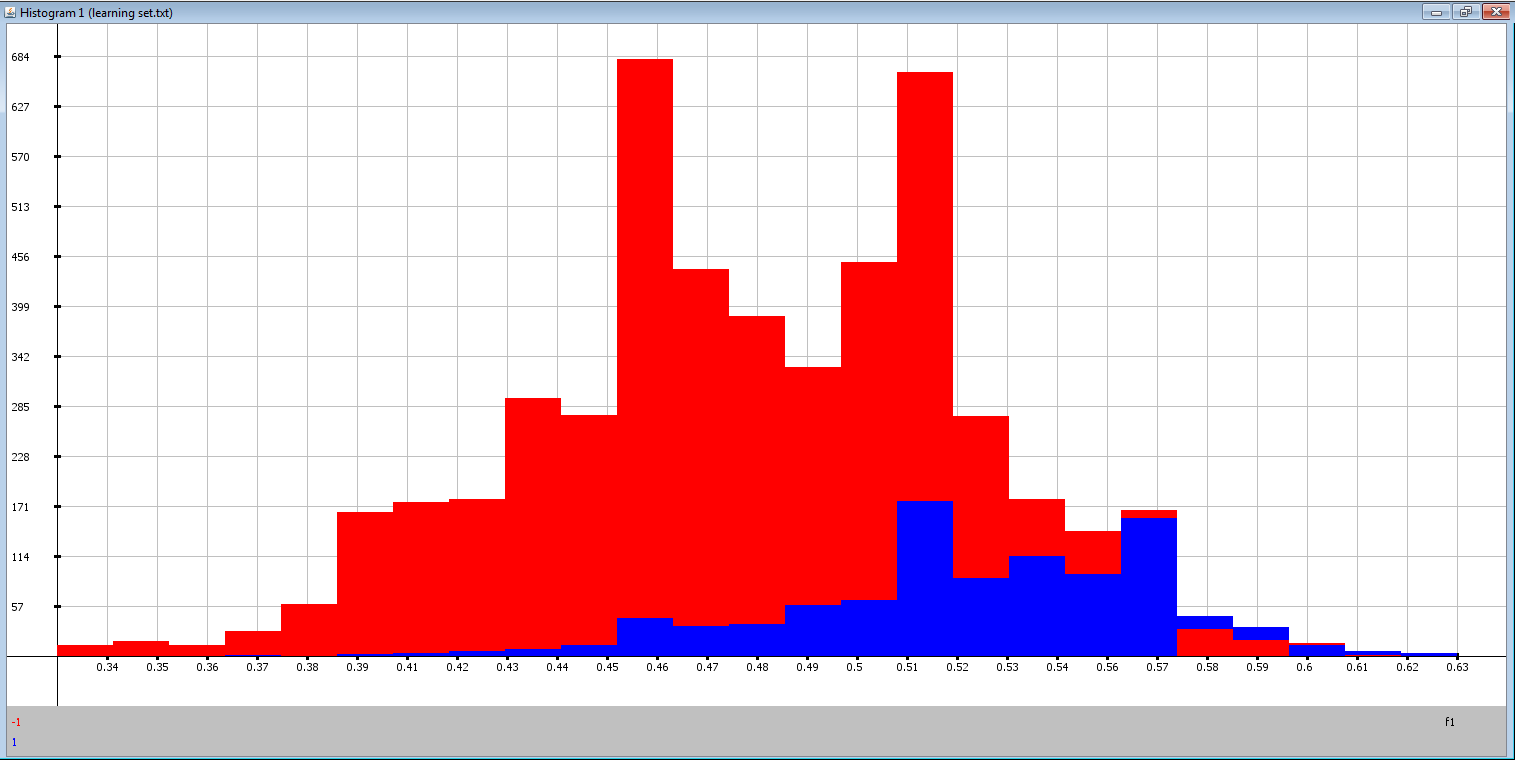
\includegraphics[width=260pt]{s8.png}
\end{figure} 

\newpage
Trend of feature m1 for classes 1 and -1:

\begin{figure}[htb]
\centering
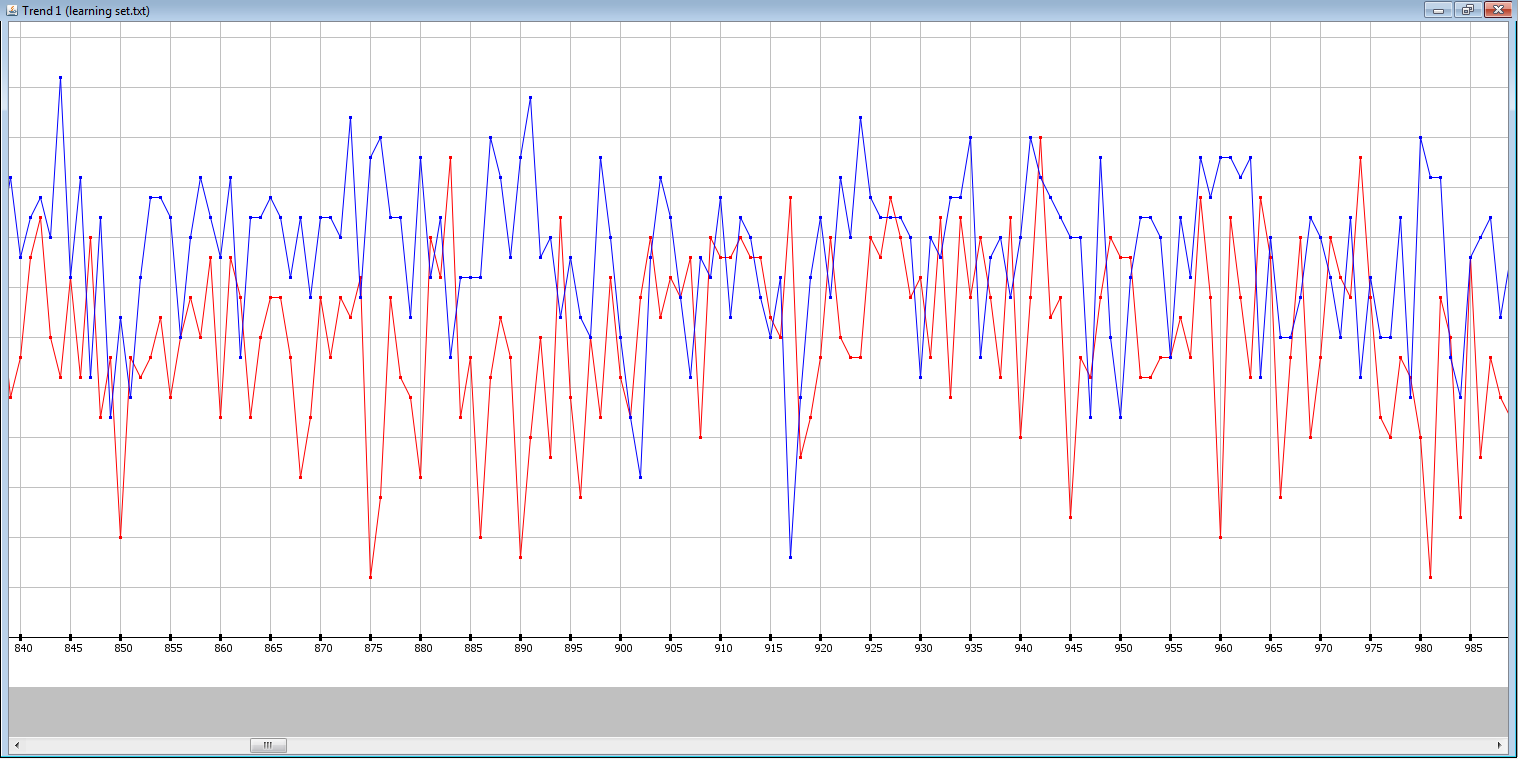
\includegraphics[width=320pt]{s9.png}
\end{figure} 

3D Plot of features m1, m2, and m3 for classes 1 and -1:

\begin{figure}[htb]
\centering
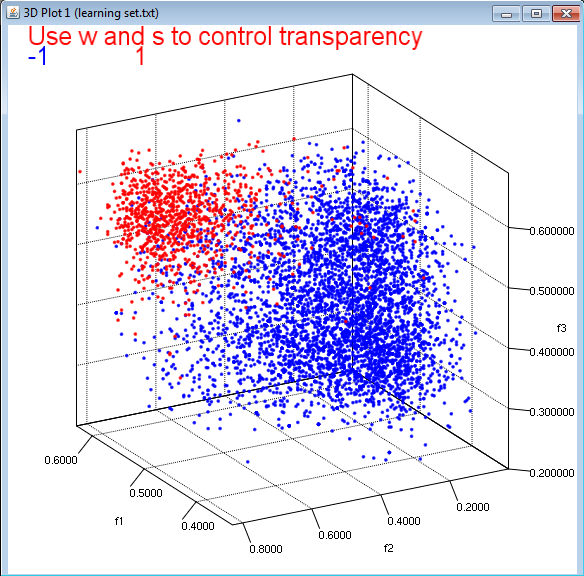
\includegraphics[width=260pt]{s10.png}
\end{figure}

\newpage

\section*{Classification}
\addcontentsline{toc}{section}{Classification}
Following data classification methods are available:
\begin{enumerate}
\item	Linear and Quadratic Discriminant Analysis.
\item Neural Net 
\item Least Squares 
\item Nearest Neighbors
\end{enumerate}
They are all available in menu Classification. 
\subsection*{LDF and QDF}
\addcontentsline{toc}{subsection}{LDF and QDF}
To choose between linear and quadratic analysis use menu Options/DA Options. Also, you can select if the method should use the prior probability which is selected by default. Go to Classification/DA analysis and press analyze. After analyzing the data you can draw accuracy histogram to manually change the decision threshold and see how good the method performs. 
 
\begin{figure}[htb]
\centering
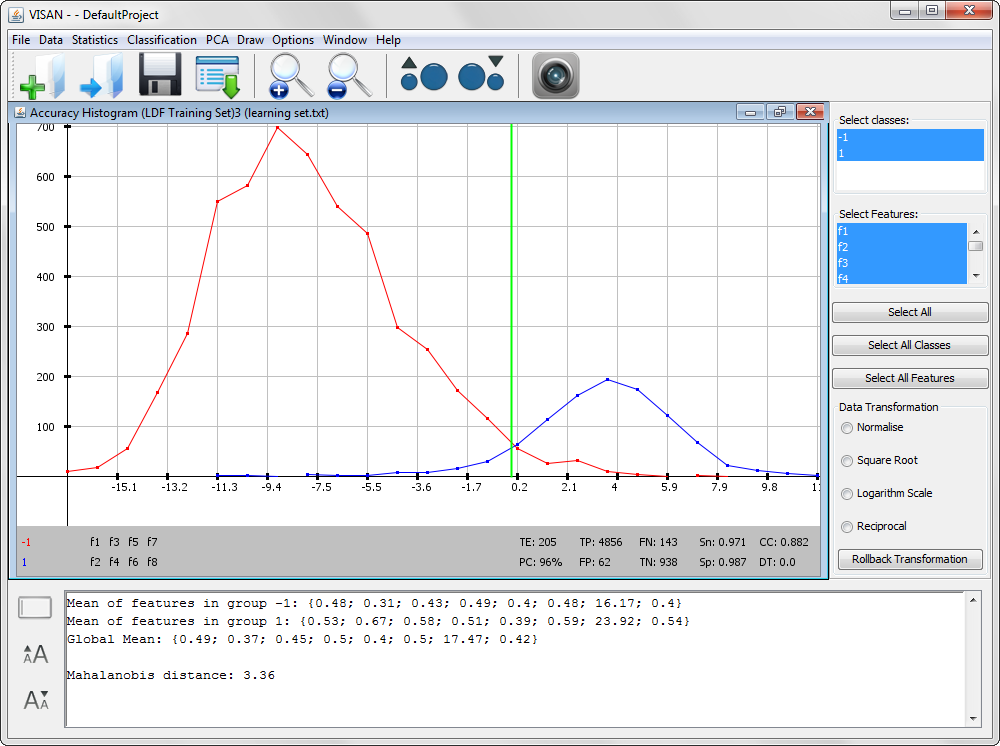
\includegraphics[width=360pt]{s11.png}
\caption{Accuracy Histogram}
\end{figure}
\newpage
Use classify to find out classes for new unlabeled data. Example of input for classification:

\begin{lstlisting}
0.50    0.40    0.45    0.51    0.36    0.41   18.00    0.10  
0.50    0.69    0.57    0.53    0.64    0.74   18.00    0.54   
\end{lstlisting}

The features should obviously be in same order as original learning set. 


If you also have testing set for your data you can draw testing set histogram. You can see how good the algorithm performs on testing set. Select Test histogram and select the testing set file.

\begin{figure}[htb]
\centering
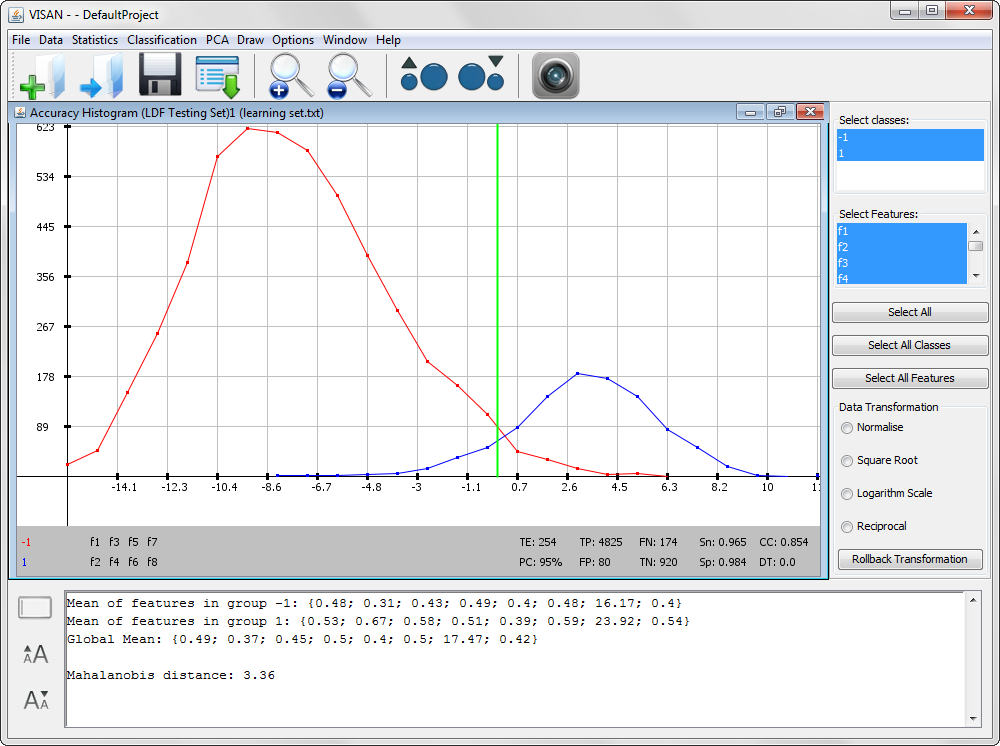
\includegraphics[width=360pt]{s12.png}
\caption{Testing set Histogram}
\end{figure}

Testing set should not have features names in it. Example:

\begin{lstlisting}
0.59    0.38    0.52    0.50    0.34    0.49   25.00    0.44  -1
0.47    0.53    0.63    0.50    0.37    0.43   19.00    0.41  -1
0.44    0.39    0.50    0.50    0.34    0.50   13.00    0.38   1
0.57    0.21    0.35    0.45    0.37    0.30   12.00    0.36  -1
\end{lstlisting}


Histogram, test histogram and classify work same for all methods.

\subsection*{Neural Networks}
\addcontentsline{toc}{subsection}{Neural Networks}
To use neural networks, you first need to train the network. Press "learn" in and you can see the progress in console. Neural Net has a lot of parameters that can be changed from Options/Neural Net, or the default values can be used. Most of parameters are set to optimal values and should not be changed unless you have experience with neural networks. The parameters that should be considered by user to change are stopping criteria and the number of learns.

Choose one of the stopping criteria from Options/Neural Net - "Testing Set Stop", "No Improvements Stop", or "Manual Stop".  At any time you can manually stop learning by selecting Classification/Neural Net/Stop Learning. If you want to obtain very good neural net for classification, set the number of learns to high number. In this case program will try a lot of different nets and choose the best one. Remember that you can always stop the learning and in that case the best net so far will be used. 

For example, see the figure bellow. Here we are training neural networks with number of learns set to 100 and using testing set stop. Result is the error in the testing set for the current net, minimum is the smallest error so far. 


\begin{figure}[htb]
\centering
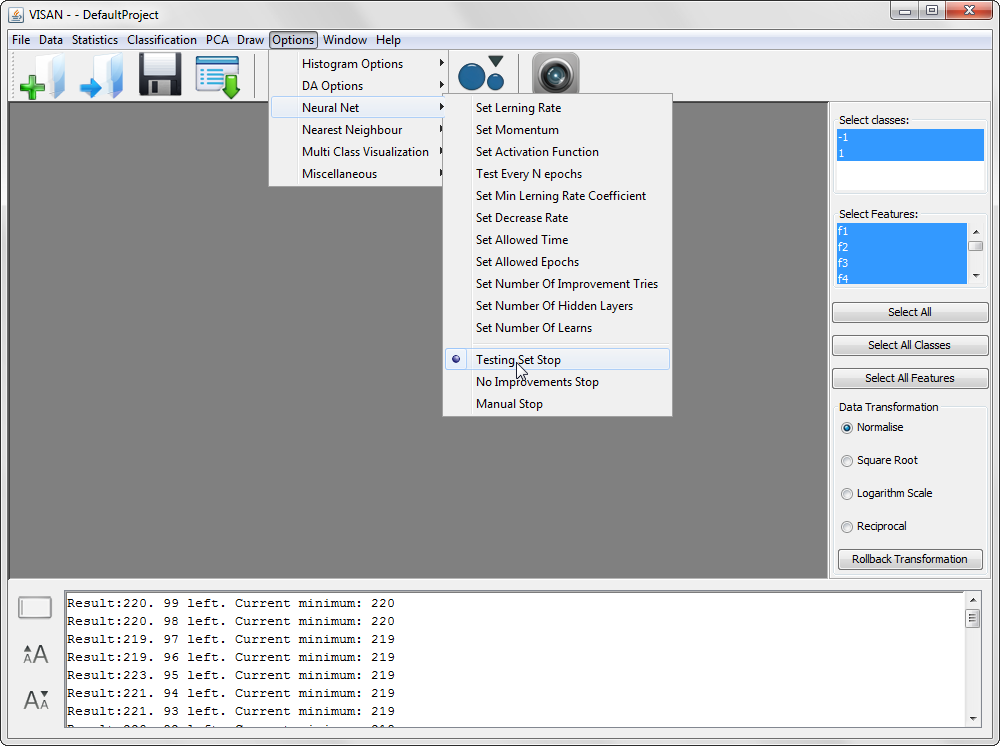
\includegraphics[width=360pt]{s13.png}
\caption{Training Neural Networks}
\end{figure}

\newpage
\subsection*{Least Squares}
\addcontentsline{toc}{subsection}{Least Squares}
Least Squares method in primary form produces results that are similar to LDF. However, it only works for two classes. Press Find Parameters first and then you can start using this method for accuracy histograms and classification. If you want to use dual form, select Options/LS Options/Dual Form. Dialog will be shown where you can select type of kernel (dot product, polynomial, or radial). Use dual form when you have a lot of features, but not many training examples. Using this method with large data sets, for example 2000 objects, may cause program to run out of memory.

\begin{figure}[htb]
\centering
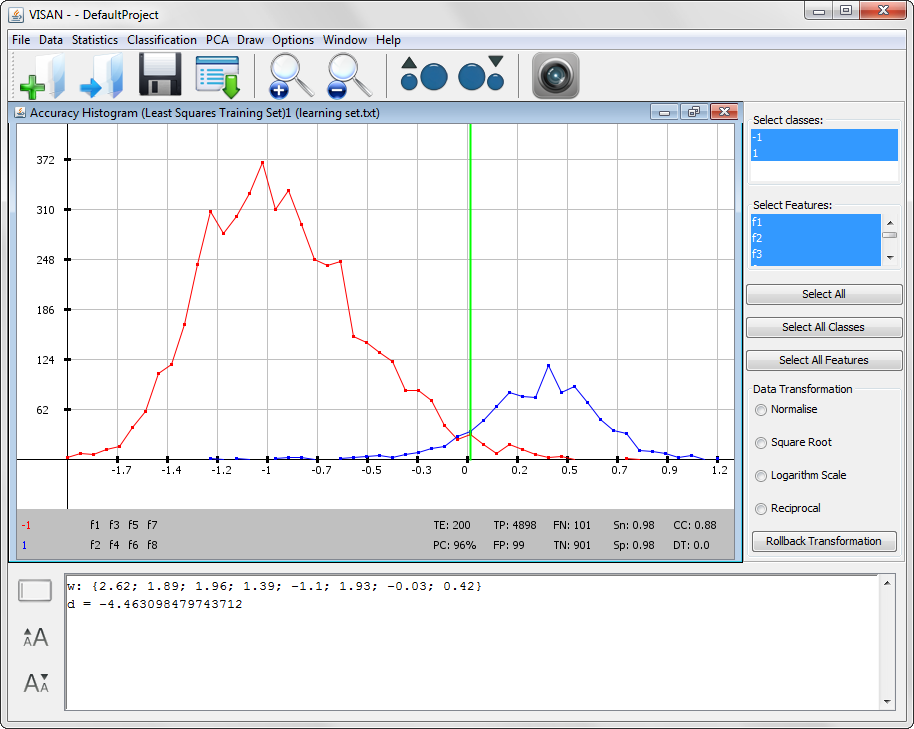
\includegraphics[width=360pt]{s17.png}
\caption{Least Squares Accuracy Histogram}
\end{figure}


\subsection*{Nearest Neighbors}
\addcontentsline{toc}{subsection}{Nearest Neighbors}
This is the most simple classification method. Only testing set histogram and classify is available for it. You can change the number of neighbors to compare to in Options/Nearest Neighbors/Choose N. Also, you can use kernelised version of nearest neighbors by selecting dual form checkbox there. 
\newpage
\section*{Principal Component Analysis}
\addcontentsline{toc}{section}{Principal Component Analysis}
Program includes Principal Component Analysis. To start using it you need to find principal components (PCA/Find Principal Components). After that you can draw 2D or 3D graph to see clustering of data. You will be prompted which eigenvectors to use. Left click on eigenvectors holding down Cntrl to choose the ones you want. They are sorted by their eigenvalue, eigenvector 0 has highest eigenvalue.

\begin{figure}[htb]
\centering
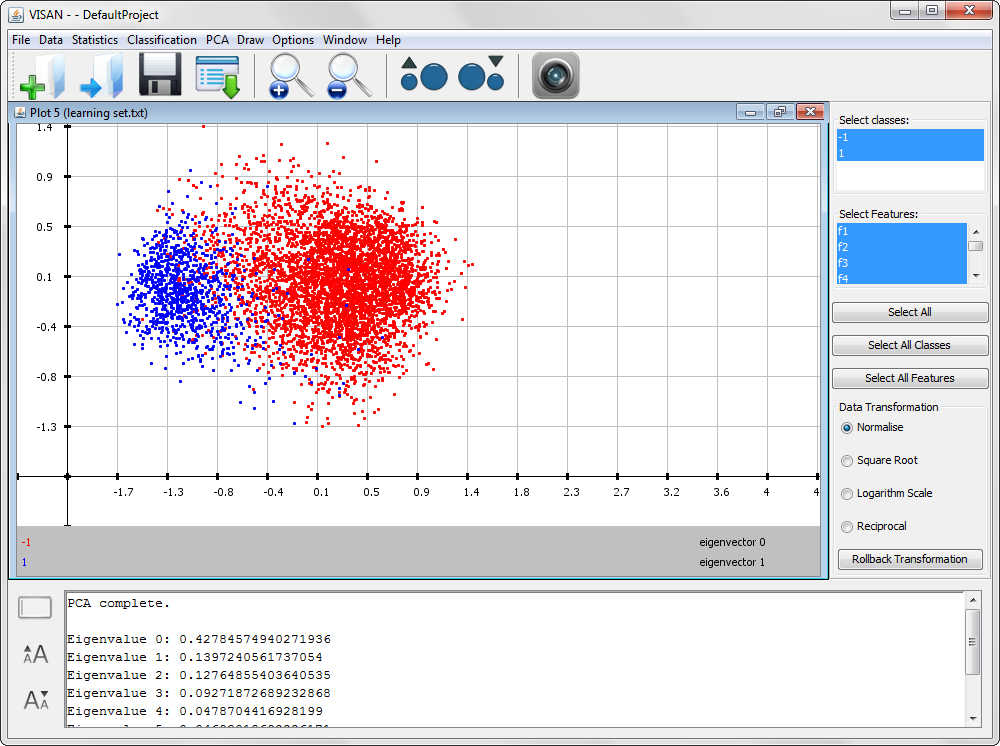
\includegraphics[width=240pt]{s15.png}
\caption{2 eigenvectors}
\end{figure}

\begin{figure}[htb]
\centering
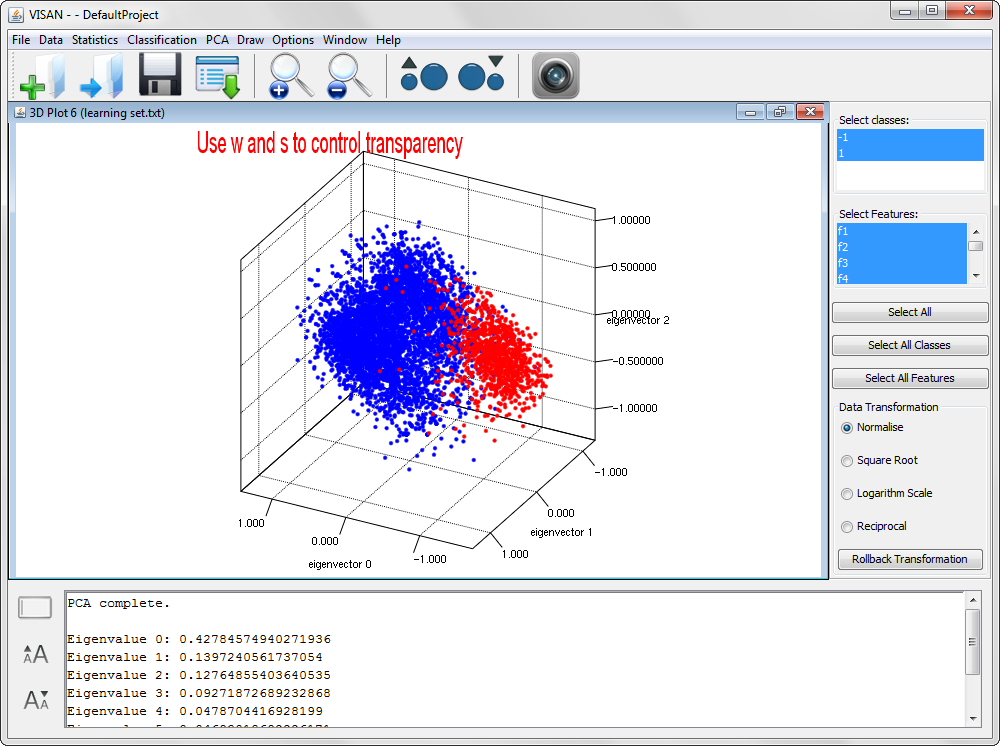
\includegraphics[width=240pt]{s16.png}
\caption{3 eigenvectors}
\end{figure}
\end{document}